\documentclass[border=10pt]{standalone}
\usepackage{tikz}


\usetikzlibrary{shapes}



\begin{document}
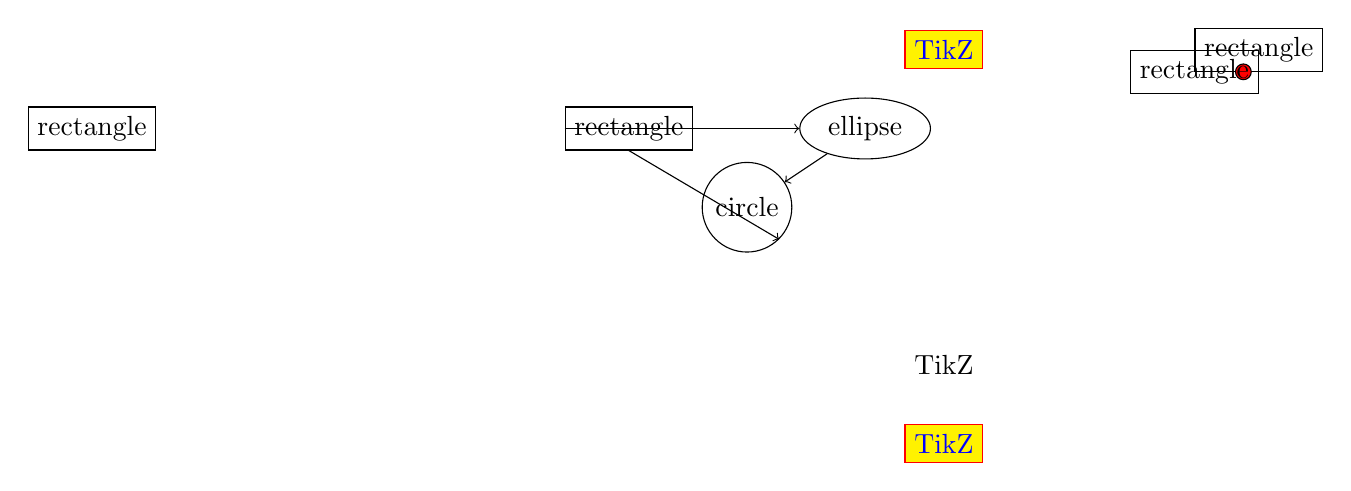
\begin{tikzpicture}
    \draw (4,2) node[draw, color=red, fill=yellow, text=blue] {TikZ};
    \node at (4,-2) {TikZ};%zonder het ingeven van die at doet de opgegeven coordinaat niks
    \node[draw, color=red, fill=yellow, text=blue] at (4,-3) {TikZ};


    \node (r) at (0,1)   [draw] {rectangle};%default is the rectangular shape
    \node (c) at (1.5,0) [draw, circle]   {circle};
    \node (e) at (3,1)   [draw, ellipse]   {ellipse};

     \draw[->] (r.west)  -- (e);
    \draw[->] (r.south) -- (c.south east);%compass directions or anchors
    \draw[->] (e) -- (c);
    
    \node (huh) at (8,2) [draw, rectangle] {rectangle};
    \draw (huh.235) circle[radius=0.1][fill=red];
    \node at (8,2) [draw, rectangle, anchor=north  east]{rectangle};

    \node (puntje) at (-6,1)   [draw, coordinate]   {ellipse};
    \node at (puntje) [draw, rectangle, anchor=0]{rectangle};


\end{tikzpicture}
\end{document}